\documentclass[12pt]{article}\usepackage[]{graphicx}\usepackage[]{color}
%% maxwidth is the original width if it is less than linewidth
%% otherwise use linewidth (to make sure the graphics do not exceed the margin)
\makeatletter
\def\maxwidth{ %
  \ifdim\Gin@nat@width>\linewidth
    \linewidth
  \else
    \Gin@nat@width
  \fi
}
\makeatother

\definecolor{fgcolor}{rgb}{0.345, 0.345, 0.345}
\newcommand{\hlnum}[1]{\textcolor[rgb]{0.686,0.059,0.569}{#1}}%
\newcommand{\hlstr}[1]{\textcolor[rgb]{0.192,0.494,0.8}{#1}}%
\newcommand{\hlcom}[1]{\textcolor[rgb]{0.678,0.584,0.686}{\textit{#1}}}%
\newcommand{\hlopt}[1]{\textcolor[rgb]{0,0,0}{#1}}%
\newcommand{\hlstd}[1]{\textcolor[rgb]{0.345,0.345,0.345}{#1}}%
\newcommand{\hlkwa}[1]{\textcolor[rgb]{0.161,0.373,0.58}{\textbf{#1}}}%
\newcommand{\hlkwb}[1]{\textcolor[rgb]{0.69,0.353,0.396}{#1}}%
\newcommand{\hlkwc}[1]{\textcolor[rgb]{0.333,0.667,0.333}{#1}}%
\newcommand{\hlkwd}[1]{\textcolor[rgb]{0.737,0.353,0.396}{\textbf{#1}}}%

\usepackage{framed}
\makeatletter
\newenvironment{kframe}{%
 \def\at@end@of@kframe{}%
 \ifinner\ifhmode%
  \def\at@end@of@kframe{\end{minipage}}%
  \begin{minipage}{\columnwidth}%
 \fi\fi%
 \def\FrameCommand##1{\hskip\@totalleftmargin \hskip-\fboxsep
 \colorbox{shadecolor}{##1}\hskip-\fboxsep
     % There is no \\@totalrightmargin, so:
     \hskip-\linewidth \hskip-\@totalleftmargin \hskip\columnwidth}%
 \MakeFramed {\advance\hsize-\width
   \@totalleftmargin\z@ \linewidth\hsize
   \@setminipage}}%
 {\par\unskip\endMakeFramed%
 \at@end@of@kframe}
\makeatother

\definecolor{shadecolor}{rgb}{.97, .97, .97}
\definecolor{messagecolor}{rgb}{0, 0, 0}
\definecolor{warningcolor}{rgb}{1, 0, 1}
\definecolor{errorcolor}{rgb}{1, 0, 0}
\newenvironment{knitrout}{}{} % an empty environment to be redefined in TeX

\usepackage{alltt}
\usepackage{amsmath,amsfonts}
\usepackage{hyperref}
\usepackage{geometry}
 \geometry{
 letterpaper,
 left=15mm,
 right=15mm,
 top=20mm,
 bottom=20mm,
 }
\usepackage[affil-it]{authblk}

%\sectionfont{\fontsize{14}{20}\selectfont}  % must have \selectfont to make the font change happen



\IfFileExists{upquote.sty}{\usepackage{upquote}}{}
\begin{document}
  \title{Work Summary and Prospective Plan}
  \author{Kejun He}
  % \affil{Department of Statistics 
    % \\ Texas A{\fontshape{n}\selectfont \&}M University
  %   }
  \date{}

  \maketitle
  
  From Oct to the end of November 2014, I was working on reproducing the statistical graphs and results from \textit{A metagenomic study of diet-dependent interaction between gut microbiota and host in infants reveals differences in immune response}, authored by Scott Schwartz. This part of the work processes pretty well and it has been almost done. I am grateful to Jason and Dr.~Ivanov for their generous help and constructive suggestions.   \\ $ $ \par
However, since the Scott's gene list of \textit{Intestinal} is missing and some variables are not defined in the script, some results can not be totally reproduced. In addition, there is no ``\texttt{set.seed()}'' for the generation of randomness in the script which makes some reproduced plots look different from the paper's. Moreover, the CCA part of Scott's paper did not use sparse structure, thus the gene selection is questionable. Therefore, I turn to the direction based on sparse CCA, and the tuning parameter sparsity is chosen with most significant value from permutation. As a result, my gene selection from \textit{Immunology} consists of \texttt{CD40, SEMA4D, TACR1, HLA-DOB, CCL22, CD9, GSTM4, CCL18, LRRC8E, SNED1} based on the first component score, which is different from Scott's gene selection list on his page 8. And the 5 most ``correlated'' microbial species include ``\texttt{Virulence - Resistance to antibiotics and toxic compounds, Virulence - Virulence, Cell Wall and Capsule - Capsular and extracellular polysacchrides, Respiration - Electron donating reactions, Carbohydrates - Aminosugars}''
\begin{knitrout}
\definecolor{shadecolor}{rgb}{0.969, 0.969, 0.969}\color{fgcolor}

{\centering 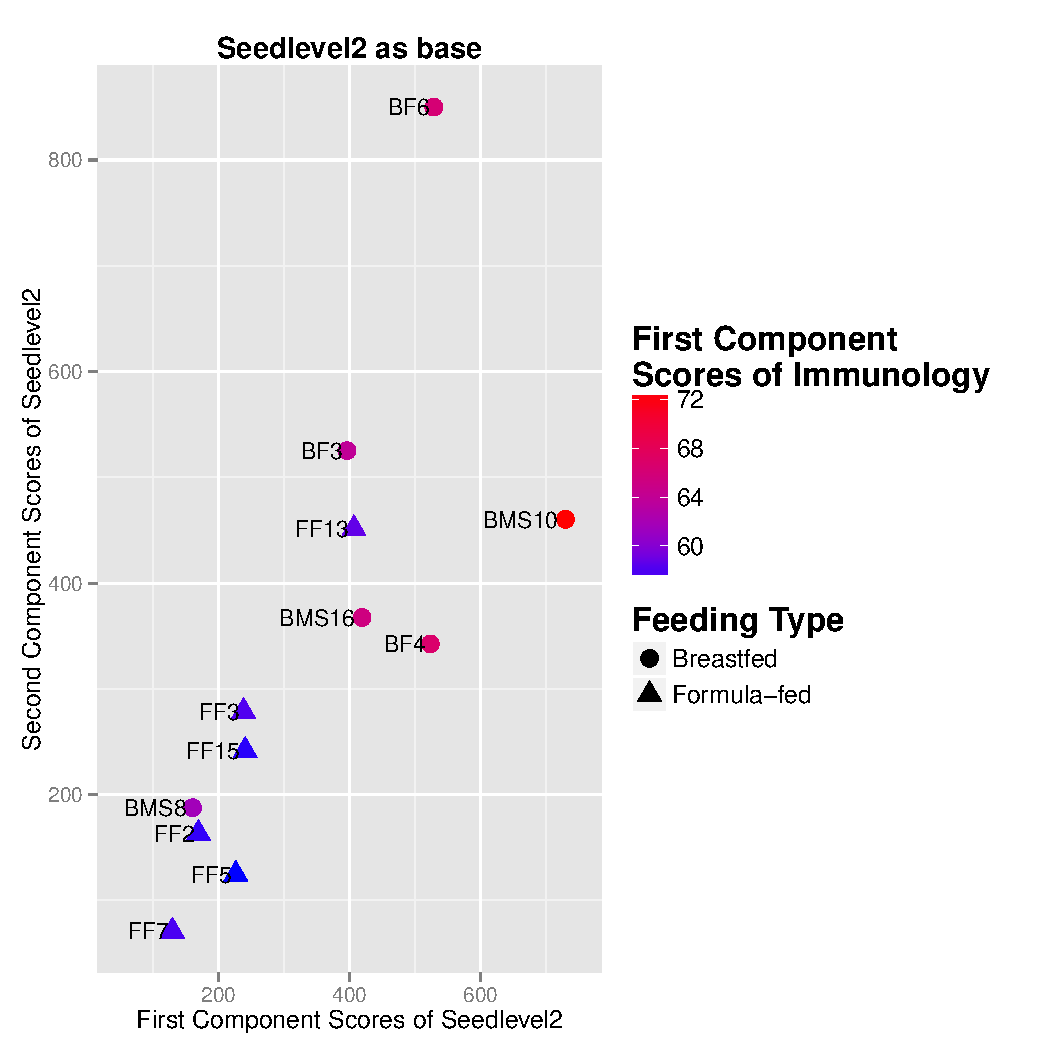
\includegraphics[width=9.2cm,height=6.5cm]{figure/plot-1} 
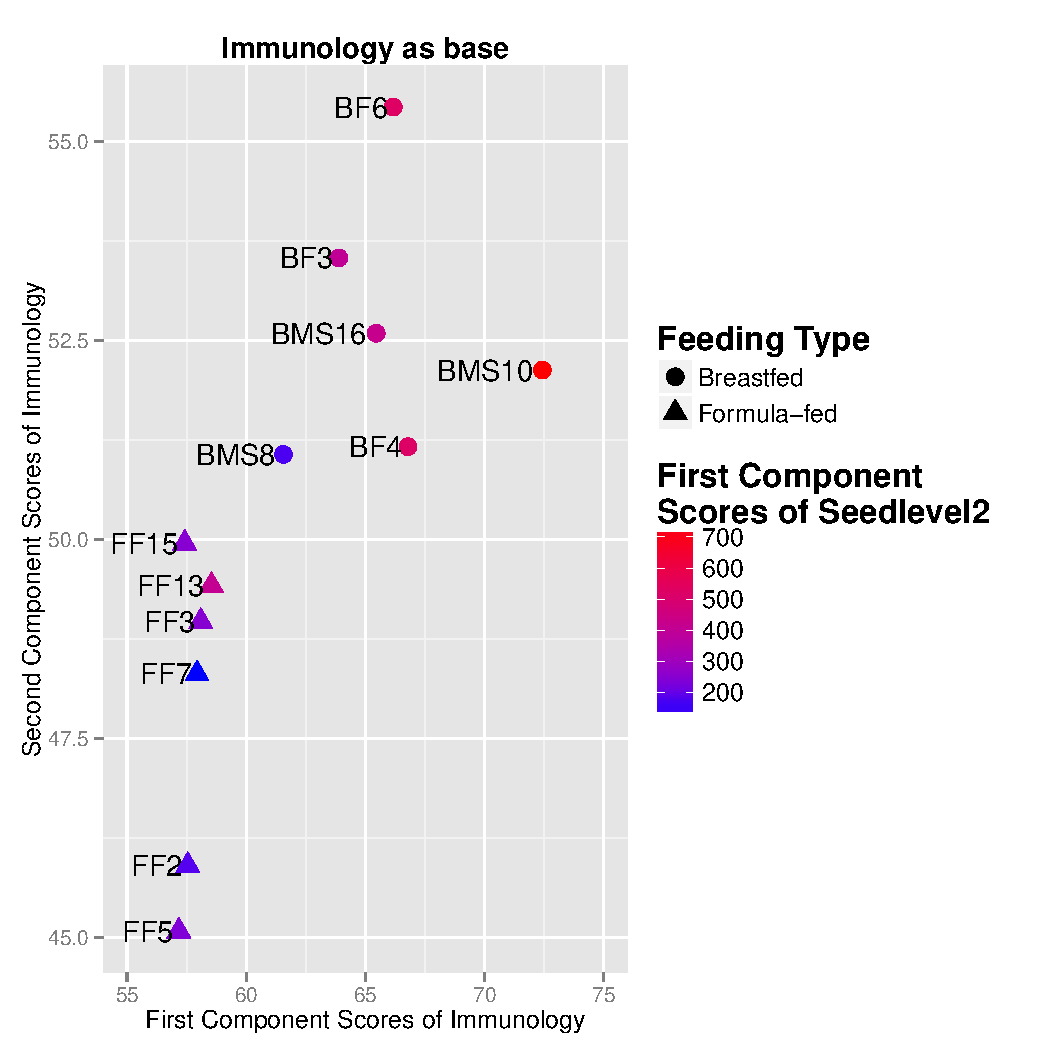
\includegraphics[width=9.2cm,height=6.5cm]{figure/plot-2} 

}



\end{knitrout}
The first plot above shows each subject on the base of \textit{first and second components scores of Seedlevel2} microbial community with different colors describing the first component scores of \textit{Immunology} and different shapes based on the difference of feeding types. And the second plot above shows the difference when we select the top 5 Seedlevel species as well.   \\  $ $ \par
In future, I am gonna work with Dr.~Qian to improve the CCA methodology, and our main approach may take into account the group structures, such as graph Laplacian,  and proportional data constraints.

\begin{knitrout}
\definecolor{shadecolor}{rgb}{0.969, 0.969, 0.969}\color{fgcolor}\begin{kframe}
\begin{alltt}
\hlcom{## redo the sparse CCA with permuted best penalties choises.}
\hlkwd{library}\hlstd{(PMA)}
\hlstd{cca_permute_both}\hlkwb{<-}\hlkwd{CCA.permute}\hlstd{(}\hlkwc{x}\hlstd{=cca_seed2,}\hlkwc{z}\hlstd{=cca_microarray_subjects,}
                          \hlkwc{typex}\hlstd{=}\hlstr{"standard"}\hlstd{,}\hlkwc{typez}\hlstd{=}\hlstr{"standard"}\hlstd{,}\hlkwc{nperms}\hlstd{=}\hlnum{30}\hlstd{)}
\end{alltt}
\end{kframe}
\begin{kframe}\begin{alltt}
\hlstd{pen_x}\hlkwb{<-}\hlstd{cca_permute_both}\hlopt{$}\hlstd{bestpenaltyx}
\hlstd{pen_z}\hlkwb{<-}\hlstd{cca_permute_both}\hlopt{$}\hlstd{bestpenaltyz}
\hlstd{cca_out_both_2}\hlkwb{<-}\hlkwd{CCA}\hlstd{(}\hlkwc{x}\hlstd{=cca_seed2,}\hlkwc{z}\hlstd{=cca_microarray_subjects,}
                  \hlkwc{typex}\hlstd{=}\hlstr{"standard"}\hlstd{,}\hlkwc{typez}\hlstd{=}\hlstr{"standard"}\hlstd{,}
                  \hlkwc{penaltyx}\hlstd{=pen_x,}\hlkwc{penaltyz}\hlstd{=pen_z,}
                  \hlkwc{xnames}\hlstd{=}\hlkwd{abbreviate}\hlstd{(}\hlkwd{colnames}\hlstd{(cca_seed2),}\hlkwc{min}\hlstd{=}\hlnum{20}\hlstd{),}
                 \hlkwc{znames}\hlstd{=}\hlkwd{colnames}\hlstd{(cca_microarray_subjects),}
                 \hlkwc{K}\hlstd{=}\hlnum{2}\hlstd{)}
\end{alltt}
\begin{verbatim}
## 123456789101112131415
## 123456789101112131415
\end{verbatim}
\begin{alltt}
\hlcom{#cca_out_both$u}
\hlstd{cca_scores_u_2}\hlkwb{<-}\hlstd{cca_seed2}\hlopt\hlstd{cca_out_both_2}\hlopt{$}\hlstd{u}
\hlstd{cca_scores_v_2}\hlkwb{<-}\hlstd{cca_microarray_subjects}\hlopt\hlstd{cca_out_both_2}\hlopt{$}\hlstd{v}
\hlstd{cca_scores_2}\hlkwb{<-}\hlkwd{cbind}\hlstd{(cca_scores_u_2,cca_scores_v_2)}
\hlkwd{colnames}\hlstd{(cca_scores_2)}\hlkwb{<-}\hlkwd{c}\hlstd{(}\hlstr{"U1"}\hlstd{,}\hlstr{"U2"}\hlstd{,}\hlstr{"V1"}\hlstd{,}\hlstr{"V2"}\hlstd{)}
\hlstd{cca_scores_2}\hlkwb{<-}\hlkwd{as.data.frame}\hlstd{(cca_scores_2)}
\hlstd{cca_scores_2}\hlopt{$}\hlstd{type}\hlkwb{<-}\hlkwd{c}\hlstd{(}\hlkwd{rep}\hlstd{(}\hlstr{"BF"}\hlstd{,}\hlnum{6}\hlstd{),}\hlkwd{rep}\hlstd{(}\hlstr{"FF"}\hlstd{,}\hlnum{6}\hlstd{))}

\hlkwd{library}\hlstd{(ggplot2)}
\hlstd{myplot2_2}\hlkwb{<-}\hlkwd{ggplot}\hlstd{(cca_scores_2,}\hlkwd{aes}\hlstd{(}\hlkwc{x}\hlstd{=V1,}\hlkwc{y}\hlstd{=V2,}\hlkwc{col}\hlstd{=U1,}\hlkwc{shape}\hlstd{=type))}
\hlstd{myplot2_2}\hlkwb{<-}\hlstd{myplot2_2}\hlopt{+}\hlkwd{geom_point}\hlstd{(}\hlkwc{size}\hlstd{=}\hlnum{4}\hlstd{)}
\hlstd{myplot2_2}\hlkwb{<-}\hlstd{myplot2_2}\hlopt{+}\hlkwd{scale_colour_continuous}\hlstd{(}\hlkwc{name}\hlstd{=}\hlstr{"First Component\textbackslash{}nScores of Seedlevel2"}\hlstd{,}
                                         \hlkwc{low}\hlstd{=}\hlstr{"blue"}\hlstd{,}\hlkwc{high}\hlstd{=}\hlstr{"red"}\hlstd{)}
\hlstd{myplot2_2}\hlkwb{<-}\hlstd{myplot2_2}\hlopt{+}\hlkwd{scale_shape_discrete}\hlstd{(}\hlkwc{name}\hlstd{=}\hlstr{"Feeding Type"}\hlstd{,}
                                      \hlkwc{labels}\hlstd{=}\hlkwd{c}\hlstd{(}\hlstr{"Breastfed"}\hlstd{,}\hlstr{"Formula-fed"}\hlstd{))}
\hlstd{myplot2_2}\hlkwb{<-}\hlstd{myplot2_2}\hlopt{+}\hlkwd{geom_text}\hlstd{(}\hlkwd{aes}\hlstd{(}\hlkwc{label}\hlstd{=}\hlkwd{rownames}\hlstd{(cca_scores_2)),}\hlkwc{col}\hlstd{=}\hlstr{"black"}\hlstd{,}\hlkwc{hjust}\hlstd{=}\hlnum{1.1}\hlstd{,}\hlkwc{size}\hlstd{=}\hlnum{5}\hlstd{)}
\hlstd{myplot2_2}\hlkwb{<-}\hlstd{myplot2_2}\hlopt{+}\hlkwd{scale_x_continuous}\hlstd{(}\hlstr{"First Component Scores of Immunology"}\hlstd{,}
                                        \hlkwc{limits}\hlstd{=}\hlkwd{c}\hlstd{(}\hlnum{55}\hlstd{,}\hlnum{75}\hlstd{))}
\hlstd{myplot2_2}\hlkwb{<-}\hlstd{myplot2_2}\hlopt{+}\hlkwd{scale_y_continuous}\hlstd{(}\hlstr{"Second Component Scores of Immunology"}\hlstd{)}
\hlstd{myplot2_2}\hlkwb{<-}\hlstd{myplot2_2}\hlopt{+}\hlkwd{labs}\hlstd{(}\hlkwc{title}\hlstd{=}\hlstr{"Sparse CCA Scores for Immunology as Base"}\hlstd{)}
\hlstd{myplot2_2}\hlkwb{<-}\hlstd{myplot2_2}\hlopt{+}\hlkwd{theme}\hlstd{(}\hlkwc{legend.title} \hlstd{=} \hlkwd{element_text}\hlstd{(}\hlkwc{size}\hlstd{=}\hlnum{12}\hlstd{),}
                       \hlkwc{plot.title} \hlstd{=} \hlkwd{element_text}\hlstd{(}\hlkwc{size}\hlstd{=}\hlnum{16}\hlstd{,}\hlkwc{vjust}\hlstd{=}\hlnum{2.0}\hlstd{,} \hlkwc{face}\hlstd{=}\hlstr{"bold"}\hlstd{),}
                       \hlkwc{legend.text}\hlstd{=}\hlkwd{element_text}\hlstd{(}\hlkwc{size}\hlstd{=}\hlnum{10}\hlstd{))}
\hlkwd{setInternet2}\hlstd{(T)} \hlcom{## to make https work}
\hlkwd{source}\hlstd{(}\hlstr{"https://raw.githubusercontent.com/low-decarie/FAAV/master/r/stat-ellipse.R"}\hlstd{)}
\hlstd{myplot2_2}\hlkwb{<-}\hlstd{myplot2_2}\hlopt{+}\hlkwd{stat_ellipse}\hlstd{(}\hlkwd{aes}\hlstd{(}\hlkwc{fill}\hlstd{=type),}\hlkwc{level}\hlstd{=}\hlnum{0.85}\hlstd{,}\hlkwc{alpha}\hlstd{=}\hlnum{0.2}\hlstd{,}
                                  \hlkwc{geom}\hlstd{=}\hlstr{"polygon"}\hlstd{,}\hlkwc{linetype}\hlstd{=}\hlnum{2}\hlstd{)}
\hlcom{#level for the scale of elli, alpha for the darkness of col,"polygon" for the cover of elli.}
\hlcom{#linetype=2 make the boundary transparent.}
\hlstd{myplot2_2}\hlkwb{<-}\hlstd{myplot2_2}\hlopt{+}\hlkwd{scale_fill_discrete}\hlstd{(}\hlkwc{name}\hlstd{=}\hlstr{"Feeding Type"}\hlstd{,}
                                      \hlkwc{labels}\hlstd{=}\hlkwd{c}\hlstd{(}\hlstr{"Breastfed"}\hlstd{,}\hlstr{"Formula-fed"}\hlstd{))}
\hlstd{myplot2_2}
\end{alltt}
\end{kframe}
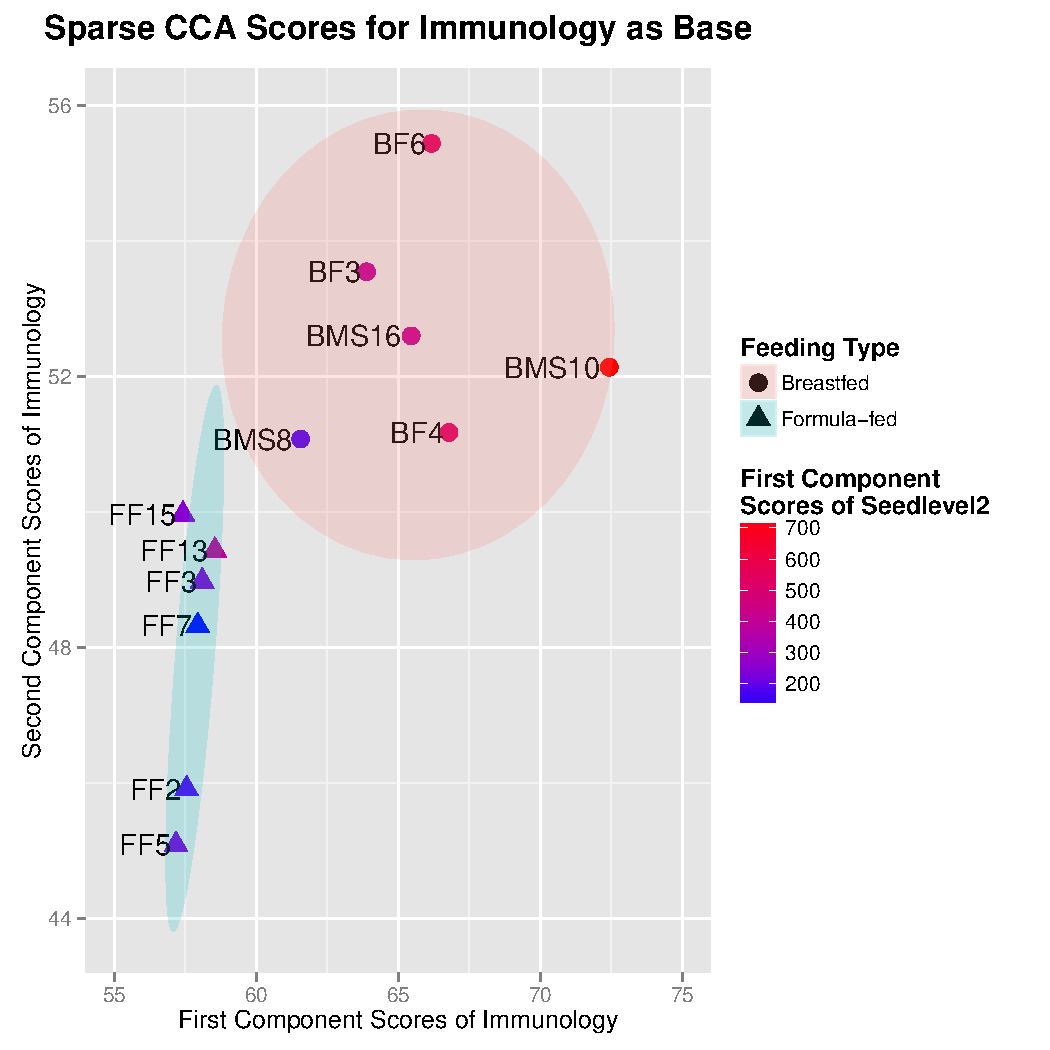
\includegraphics[width=\maxwidth]{figure/plot2-1} 
\begin{kframe}\begin{alltt}
\hlstd{myplot1_2}\hlkwb{<-}\hlkwd{ggplot}\hlstd{(cca_scores_2,}\hlkwd{aes}\hlstd{(}\hlkwc{x}\hlstd{=U1,}\hlkwc{y}\hlstd{=U2,}\hlkwc{col}\hlstd{=V1,}\hlkwc{shape}\hlstd{=type))}
\hlstd{myplot1_2}\hlkwb{<-}\hlstd{myplot1_2}\hlopt{+}\hlkwd{geom_point}\hlstd{(}\hlkwc{size}\hlstd{=}\hlnum{4}\hlstd{)}
\hlstd{myplot1_2}\hlkwb{<-}\hlstd{myplot1_2}\hlopt{+}\hlkwd{scale_colour_continuous}\hlstd{(}\hlkwc{name}\hlstd{=}\hlstr{"First Component\textbackslash{}nScores of Immunology"}\hlstd{,}
                                         \hlkwc{low}\hlstd{=}\hlstr{"blue"}\hlstd{,}\hlkwc{high}\hlstd{=}\hlstr{"red"}\hlstd{)}
\hlstd{myplot1_2}\hlkwb{<-}\hlstd{myplot1_2}\hlopt{+}\hlkwd{scale_shape_discrete}\hlstd{(}\hlkwc{name}\hlstd{=}\hlstr{"Feeding Type"}\hlstd{,}
                                      \hlkwc{labels}\hlstd{=}\hlkwd{c}\hlstd{(}\hlstr{"Breastfed"}\hlstd{,}\hlstr{"Formula-fed"}\hlstd{))}
\hlstd{myplot1_2}\hlkwb{<-}\hlstd{myplot1_2}\hlopt{+}\hlkwd{geom_text}\hlstd{(}\hlkwd{aes}\hlstd{(}\hlkwc{label}\hlstd{=}\hlkwd{rownames}\hlstd{(cca_scores)),}\hlkwc{col}\hlstd{=}\hlstr{"black"}\hlstd{,}\hlkwc{hjust}\hlstd{=}\hlnum{1.1}\hlstd{,}\hlkwc{size}\hlstd{=}\hlnum{4}\hlstd{)}
\hlstd{myplot1_2}\hlkwb{<-}\hlstd{myplot1_2}\hlopt{+}\hlkwd{scale_x_continuous}\hlstd{(}\hlstr{"First Component Scores of Seedlevel2"}\hlstd{,}
                                        \hlkwc{limits}\hlstd{=}\hlkwd{c}\hlstd{(}\hlnum{100}\hlstd{,}\hlnum{750}\hlstd{))}
\hlstd{myplot1_2}\hlkwb{<-}\hlstd{myplot1_2}\hlopt{+}\hlkwd{scale_y_continuous}\hlstd{(}\hlstr{"Second Component Scores of Seedlevel2"}\hlstd{)}
\hlstd{myplot1_2}\hlkwb{<-}\hlstd{myplot1_2}\hlopt{+}\hlkwd{labs}\hlstd{(}\hlkwc{title}\hlstd{=}\hlstr{"Sparse CCA Scores for Seedlevel2 as Base"}\hlstd{)}
\hlstd{myplot1_2}\hlkwb{<-}\hlstd{myplot1_2}\hlopt{+}\hlkwd{theme}\hlstd{(}\hlkwc{legend.title} \hlstd{=} \hlkwd{element_text}\hlstd{(}\hlkwc{size}\hlstd{=}\hlnum{12}\hlstd{),}
                       \hlkwc{plot.title} \hlstd{=} \hlkwd{element_text}\hlstd{(}\hlkwc{vjust}\hlstd{=}\hlnum{2.0}\hlstd{,}\hlkwc{size}\hlstd{=}\hlnum{16}\hlstd{,} \hlkwc{face}\hlstd{=}\hlstr{"bold"}\hlstd{),}
                       \hlkwc{legend.text}\hlstd{=}\hlkwd{element_text}\hlstd{(}\hlkwc{size}\hlstd{=}\hlnum{10}\hlstd{))}
\hlstd{myplot1_2}\hlkwb{<-}\hlstd{myplot1_2}\hlopt{+}\hlkwd{stat_ellipse}\hlstd{(}\hlkwd{aes}\hlstd{(}\hlkwc{fill}\hlstd{=type),}\hlkwc{level}\hlstd{=}\hlnum{0.6}\hlstd{,}\hlkwc{alpha}\hlstd{=}\hlnum{0.2}\hlstd{,}
                                  \hlkwc{geom}\hlstd{=}\hlstr{"polygon"}\hlstd{,}\hlkwc{linetype}\hlstd{=}\hlnum{2}\hlstd{)}
\hlstd{cca_scores_special}\hlkwb{<-}\hlstd{cca_scores_2[}\hlkwd{rep}\hlstd{(}\hlnum{10}\hlstd{,}\hlnum{100}\hlstd{),]}
\hlkwa{for}\hlstd{(t} \hlkwa{in} \hlnum{1}\hlopt{:}\hlnum{100}\hlstd{)\{}
 \hlstd{cca_scores_special[t,}\hlnum{1}\hlopt{:}\hlnum{2}\hlstd{]}\hlkwb{<-}\hlstd{cca_scores_special[t,}\hlnum{1}\hlopt{:}\hlnum{2}\hlstd{]}\hlopt{+}\hlkwd{c}\hlstd{(}\hlkwd{sin}\hlstd{(t}\hlopt{*}\hlnum{2}\hlopt{*}\hlstd{pi}\hlopt{/}\hlnum{100}\hlstd{)}\hlopt{*}\hlnum{50}\hlstd{,}\hlkwd{cos}\hlstd{(t}\hlopt{*}\hlnum{2}\hlopt{*}\hlstd{pi}\hlopt{/}\hlnum{100}\hlstd{)}\hlopt{*}\hlnum{50}\hlstd{)}
\hlstd{\}}
\hlstd{myplot1_2}\hlkwb{<-}\hlstd{myplot1_2}\hlopt{+}\hlkwd{geom_polygon}\hlstd{(}\hlkwd{aes}\hlstd{(}\hlkwc{x}\hlstd{=U1,}\hlkwc{y}\hlstd{=U2,}\hlkwc{fill}\hlstd{=type),cca_scores_special,}
                                    \hlkwc{alpha}\hlstd{=}\hlnum{0.2}\hlstd{,}\hlkwc{linetype}\hlstd{=}\hlnum{0}\hlstd{)}
\hlstd{cca_scores_special2}\hlkwb{<-}\hlstd{cca_scores_2[}\hlkwd{rep}\hlstd{(}\hlnum{1}\hlstd{,}\hlnum{100}\hlstd{),]}
\hlkwa{for}\hlstd{(t} \hlkwa{in} \hlnum{1}\hlopt{:}\hlnum{100}\hlstd{)\{}
 \hlstd{cca_scores_special2[t,}\hlnum{1}\hlopt{:}\hlnum{2}\hlstd{]}\hlkwb{<-}\hlstd{cca_scores_special2[t,}\hlnum{1}\hlopt{:}\hlnum{2}\hlstd{]}\hlopt{+}\hlkwd{c}\hlstd{(}\hlkwd{sin}\hlstd{(t}\hlopt{*}\hlnum{2}\hlopt{*}\hlstd{pi}\hlopt{/}\hlnum{100}\hlstd{)}\hlopt{*}\hlnum{50}\hlstd{,}\hlkwd{cos}\hlstd{(t}\hlopt{*}\hlnum{2}\hlopt{*}\hlstd{pi}\hlopt{/}\hlnum{100}\hlstd{)}\hlopt{*}\hlnum{50}\hlstd{)}
\hlstd{\}}
\hlstd{myplot1_2}\hlkwb{<-}\hlstd{myplot1_2}\hlopt{+}\hlkwd{geom_polygon}\hlstd{(}\hlkwd{aes}\hlstd{(}\hlkwc{x}\hlstd{=U1,}\hlkwc{y}\hlstd{=U2,}\hlkwc{fill}\hlstd{=type),cca_scores_special2,}
                                    \hlkwc{alpha}\hlstd{=}\hlnum{0.2}\hlstd{,}\hlkwc{linetype}\hlstd{=}\hlnum{0}\hlstd{)}
\hlstd{myplot1_2}\hlkwb{<-}\hlstd{myplot1_2}\hlopt{+}\hlkwd{scale_fill_discrete}\hlstd{(}\hlkwc{name}\hlstd{=}\hlstr{"Feeding Type"}\hlstd{,}
                                         \hlkwc{labels}\hlstd{=}\hlkwd{c}\hlstd{(}\hlstr{"Breastfed"}\hlstd{,}\hlstr{"Formula-fed"}\hlstd{))}
\hlstd{myplot1_2}
\end{alltt}
\end{kframe}
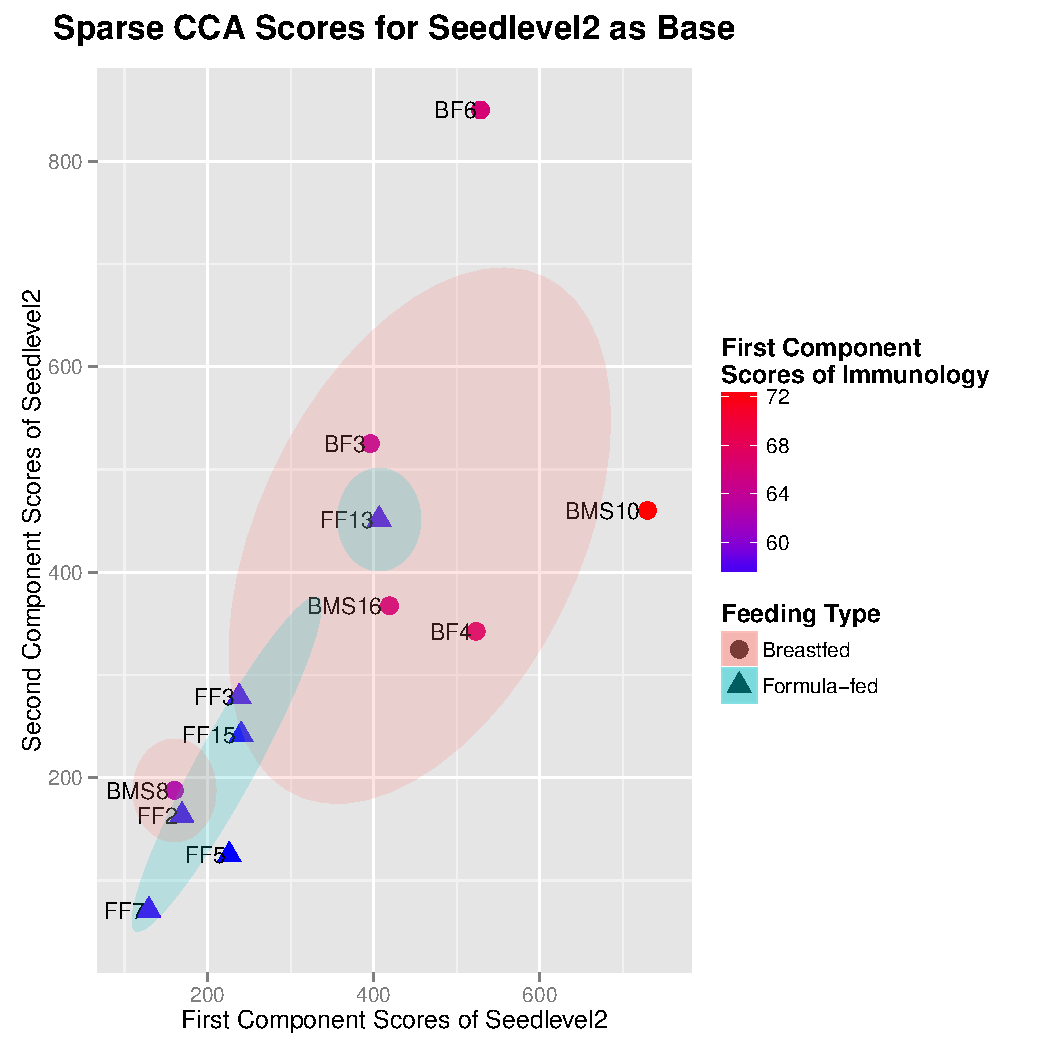
\includegraphics[width=\maxwidth]{figure/plot2-2} 
\begin{kframe}\begin{alltt}
\hlcom{## re select the names}
\hlstd{cca_seed2_t}\hlkwb{<-}\hlkwd{t}\hlstd{(cca_seed2)}
\hlstd{cca_seed2_t}\hlkwb{<-}\hlstd{cca_seed2_t}\hlopt{*}\hlstd{cca_out_both_2}\hlopt{$}\hlstd{u[,}\hlnum{1}\hlstd{]}
\hlstd{cca_seed2_tt}\hlkwb{<-}\hlkwd{t}\hlstd{(cca_seed2_t)}
\hlstd{cca_seed2_tt}\hlkwb{<-}\hlstd{cca_seed2_tt}\hlopt{*}\hlkwd{sign}\hlstd{(cca_scores_u_2[,}\hlnum{1}\hlstd{])}
\hlstd{cca_seed2_select_new}\hlkwb{<-}\hlkwd{apply}\hlstd{(cca_seed2_tt,}\hlnum{2}\hlstd{,sum)}
\hlkwd{names}\hlstd{(cca_seed2_select_new)}\hlkwb{<-}\hlkwd{colnames}\hlstd{(cca_seed2)}
\hlstd{cca_seed2_select_new_order}\hlkwb{<-}\hlkwd{sort}\hlstd{(}\hlkwd{abs}\hlstd{(cca_seed2_select_new),}\hlkwc{decreasing} \hlstd{= T)} \hlcom{# seed first compo sort}

\hlcom{## re select the microarray}
\hlstd{cca_microarray_subjects_t}\hlkwb{<-}\hlkwd{t}\hlstd{(cca_microarray_subjects)}
\hlstd{cca_microarray_subjects_t}\hlkwb{<-}\hlstd{cca_microarray_subjects_t}\hlopt{*}\hlstd{cca_out_both_2}\hlopt{$}\hlstd{v[,}\hlnum{1}\hlstd{]}
\hlstd{cca_microarray_subjects_tt}\hlkwb{<-}\hlkwd{t}\hlstd{(cca_microarray_subjects_t)}
\hlstd{cca_microarray_subjects_tt}\hlkwb{<-}\hlstd{cca_microarray_subjects_tt}\hlopt{*}\hlkwd{sign}\hlstd{(cca_scores_v_2[,}\hlnum{1}\hlstd{])}
\hlstd{cca_micro_select_new}\hlkwb{<-}\hlkwd{apply}\hlstd{(cca_microarray_subjects_tt,}\hlnum{2}\hlstd{,sum)}
\hlkwd{names}\hlstd{(cca_micro_select_new)}\hlkwb{<-}\hlkwd{colnames}\hlstd{(cca_microarray_subjects)}
\hlstd{cca_micro_select_new_order}\hlkwb{<-}\hlkwd{sort}\hlstd{(}\hlkwd{abs}\hlstd{(cca_micro_select_new),}
                                 \hlkwc{decreasing}\hlstd{=T)} \hlcom{# microarray fist compo sort}
\end{alltt}
\end{kframe}
\end{knitrout}

\begin{knitrout}
\definecolor{shadecolor}{rgb}{0.969, 0.969, 0.969}\color{fgcolor}\begin{kframe}
\begin{alltt}
\hlkwd{library}\hlstd{(PMA)}
\hlstd{spca_immun_cv}\hlkwb{<-}\hlkwd{SPC.cv}\hlstd{(}\hlkwc{x}\hlstd{=cca_microarray_subjects,}\hlkwc{sumabsvs}\hlstd{=}\hlkwd{seq}\hlstd{(}\hlnum{1.2}\hlstd{,}\hlnum{25}\hlstd{,}\hlkwc{by}\hlstd{=}\hlnum{0.2}\hlstd{),}
                      \hlkwc{nfolds}\hlstd{=}\hlnum{10}\hlstd{,}\hlkwc{niter}\hlstd{=}\hlnum{10}\hlstd{)}
\end{alltt}
\begin{verbatim}
##  Fold  1  out of  10 
##  Fold  2  out of  10 
##  Fold  3  out of  10 
##  Fold  4  out of  10 
##  Fold  5  out of  10 
##  Fold  6  out of  10 
##  Fold  7  out of  10 
##  Fold  8  out of  10 
##  Fold  9  out of  10 
##  Fold  10  out of  10
\end{verbatim}
\begin{alltt}
\hlstd{spca_immun}\hlkwb{<-}\hlkwd{SPC}\hlstd{(}\hlkwc{x}\hlstd{=cca_microarray_subjects,}\hlkwc{sumabsv}\hlstd{=spca_immun_cv}\hlopt{$}\hlstd{bestsumabsv,}
                \hlkwc{K}\hlstd{=}\hlnum{2}\hlstd{)}
\end{alltt}
\begin{verbatim}
## 1234567891011121314151617181920
## 1234567891011
\end{verbatim}
\begin{alltt}
\hlstd{spca_scores}\hlkwb{<-}\hlstd{spca_immun}\hlopt{$}\hlstd{u}
\hlkwd{rownames}\hlstd{(spca_scores)}\hlkwb{<-}\hlkwd{rownames}\hlstd{(cca_microarray_subjects)}
\hlstd{spca_scores}\hlkwb{<-}\hlkwd{as.data.frame}\hlstd{(spca_scores)}
\hlkwd{names}\hlstd{(spca_scores)}\hlkwb{<-}\hlkwd{c}\hlstd{(}\hlstr{"Host1"}\hlstd{,}\hlstr{"Host2"}\hlstd{)}
\hlstd{spca_scores}\hlopt{$}\hlstd{type}\hlkwb{<-}\hlkwd{c}\hlstd{(}\hlkwd{rep}\hlstd{(}\hlstr{"BF"}\hlstd{,}\hlnum{6}\hlstd{),}\hlkwd{rep}\hlstd{(}\hlstr{"FF"}\hlstd{,}\hlnum{6}\hlstd{))}
\hlkwd{library}\hlstd{(ggplot2)}
\hlstd{spca_plot1}\hlkwb{<-}\hlkwd{ggplot}\hlstd{(spca_scores,}\hlkwd{aes}\hlstd{(}\hlkwc{x}\hlstd{=Host1,}\hlkwc{y}\hlstd{=Host2,}\hlkwc{shape}\hlstd{=type,}\hlkwc{colour}\hlstd{=type,}
                                   \hlkwc{ymax}\hlstd{=}\hlkwd{max}\hlstd{(}\hlkwd{abs}\hlstd{(Host2))}\hlopt{*}\hlnum{1.5}\hlstd{))}
\hlstd{spca_plot1}\hlkwb{<-}\hlstd{spca_plot1}\hlopt{+}\hlkwd{geom_point}\hlstd{(}\hlkwc{size}\hlstd{=}\hlnum{4}\hlstd{)}
\hlstd{spca_plot1}\hlkwb{<-}\hlstd{spca_plot1}\hlopt{+}\hlkwd{scale_shape_discrete}\hlstd{(}\hlkwc{name}\hlstd{=}\hlstr{"Feeding Type"}\hlstd{,}
                                            \hlkwc{labels}\hlstd{=}\hlkwd{c}\hlstd{(}\hlstr{"Breastfed"}\hlstd{,}\hlstr{"Formula-fed"}\hlstd{))}
\hlstd{spca_plot1}\hlkwb{<-}\hlstd{spca_plot1}\hlopt{+}\hlkwd{scale_color_discrete}\hlstd{(}\hlkwc{name}\hlstd{=}\hlstr{"Feeding Type"}\hlstd{,}
                                            \hlkwc{labels}\hlstd{=}\hlkwd{c}\hlstd{(}\hlstr{"Breastfed"}\hlstd{,}\hlstr{"Formula-fed"}\hlstd{))}
\hlstd{spca_plot1}\hlkwb{<-}\hlstd{spca_plot1}\hlopt{+}\hlkwd{geom_text}\hlstd{(}\hlkwd{aes}\hlstd{(}\hlkwc{label}\hlstd{=}\hlkwd{rownames}\hlstd{(spca_scores)),}
                                 \hlkwc{col}\hlstd{=}\hlstr{"black"}\hlstd{,}\hlkwc{hjust}\hlstd{=}\hlnum{1.1}\hlstd{,}\hlkwc{size}\hlstd{=}\hlnum{4}\hlstd{,}
                                 \hlkwc{position}\hlstd{=}\hlkwd{position_jitter}\hlstd{(}\hlkwc{height}\hlstd{=}\hlnum{0.01}\hlstd{,}\hlkwc{width}\hlstd{=}\hlnum{0.01}\hlstd{))}
\hlcom{## the position=position_jitter(height=0.01,width=0.01) will make the material in the same group }
\hlcom{# a litter bit separate.}
\hlcom{## wihle position_dodge will separate the material between groups.}

\hlstd{spca_plot1}\hlkwb{<-}\hlstd{spca_plot1}\hlopt{+}\hlkwd{scale_x_continuous}\hlstd{(}\hlstr{"First PCA scores from Hosts"}\hlstd{,}
                                          \hlkwc{limits}\hlstd{=}\hlkwd{c}\hlstd{(}\hlopt{-}\hlnum{0.55}\hlstd{,}\hlnum{0.0}\hlstd{))}
\hlstd{spca_plot1}\hlkwb{<-}\hlstd{spca_plot1}\hlopt{+}\hlkwd{scale_y_continuous}\hlstd{(}\hlstr{"Second PCA scores from Hosts"}\hlstd{)}
\hlstd{spca_plot1}\hlkwb{<-}\hlstd{spca_plot1}\hlopt{+}\hlkwd{labs}\hlstd{(}\hlkwc{title}\hlstd{=}\hlstr{"Sparse PCA Scores from Immunology of Hosts"}\hlstd{)}
\hlstd{spca_plot1}\hlkwb{<-}\hlstd{spca_plot1}\hlopt{+}\hlkwd{theme}\hlstd{(}\hlkwc{legend.title}\hlstd{=}\hlkwd{element_text}\hlstd{(}\hlkwc{size}\hlstd{=}\hlnum{10}\hlstd{),}
                             \hlkwc{legend.text}\hlstd{=}\hlkwd{element_text}\hlstd{(}\hlkwc{size}\hlstd{=}\hlnum{8}\hlstd{),}
                             \hlkwc{plot.title}\hlstd{=}\hlkwd{element_text}\hlstd{(}\hlkwc{size}\hlstd{=}\hlnum{14}\hlstd{,}\hlkwc{vjust}\hlstd{=}\hlnum{1.1}\hlstd{,}\hlkwc{face}\hlstd{=}\hlstr{"bold"}\hlstd{))}
\hlcom{#source("https://raw.github.com/low-decarie/FAAV/master/r/stat-ellipse.R")}
\hlstd{spca_plot1}\hlkwb{<-}\hlstd{spca_plot1}\hlopt{+}\hlkwd{stat_ellipse}\hlstd{(}\hlkwd{aes}\hlstd{(}\hlkwc{x}\hlstd{=Host1,}\hlkwc{y}\hlstd{=Host2,}\hlkwc{fill}\hlstd{=type),}
                                    \hlkwc{level}\hlstd{=}\hlnum{0.8}\hlstd{,}\hlkwc{geom}\hlstd{=}\hlstr{"polygon"}\hlstd{,}\hlkwc{alpha}\hlstd{=}\hlnum{0.2}\hlstd{)}
\hlstd{spca_plot1}\hlkwb{<-}\hlstd{spca_plot1}\hlopt{+}\hlkwd{scale_fill_discrete}\hlstd{(}\hlkwc{name}\hlstd{=}\hlstr{"Feeding Type"}\hlstd{,}
                                            \hlkwc{labels}\hlstd{=}\hlkwd{c}\hlstd{(}\hlstr{"Breastfed"}\hlstd{,}\hlstr{"Formula-fed"}\hlstd{))}
\hlcom{#level for the scale of elli, alpha for the darkness of col,"polygon" for the cover of elli.}
\hlstd{spca_special}\hlkwb{<-}\hlstd{spca_scores[}\hlkwd{rep}\hlstd{(}\hlnum{6}\hlstd{,}\hlnum{100}\hlstd{),]}
\hlkwa{for}\hlstd{(t} \hlkwa{in} \hlnum{1}\hlopt{:}\hlnum{100}\hlstd{)\{}
 \hlstd{spca_special[t,}\hlnum{1}\hlopt{:}\hlnum{2}\hlstd{]}\hlkwb{<-}\hlstd{spca_special[t,}\hlnum{1}\hlopt{:}\hlnum{2}\hlstd{]}\hlopt{+}\hlkwd{c}\hlstd{(}\hlkwd{sin}\hlstd{(t}\hlopt{*}\hlnum{2}\hlopt{*}\hlstd{pi}\hlopt{/}\hlnum{100}\hlstd{)}\hlopt{/}\hlnum{40}\hlstd{,}\hlkwd{cos}\hlstd{(t}\hlopt{*}\hlnum{2}\hlopt{*}\hlstd{pi}\hlopt{/}\hlnum{100}\hlstd{)}\hlopt{/}\hlnum{40}\hlstd{)}
\hlstd{\}}
\hlstd{spca_plot1}\hlkwb{<-}\hlstd{spca_plot1}\hlopt{+}\hlkwd{geom_polygon}\hlstd{(}\hlkwd{aes}\hlstd{(}\hlkwc{x}\hlstd{=Host1,}\hlkwc{y}\hlstd{=Host2,}\hlkwc{fill}\hlstd{=type),spca_special,}
                                    \hlkwc{alpha}\hlstd{=}\hlnum{0.2}\hlstd{)}
\hlstd{spca_special2}\hlkwb{<-}\hlstd{spca_scores[}\hlkwd{rep}\hlstd{(}\hlnum{11}\hlstd{,}\hlnum{100}\hlstd{),]}
\hlkwa{for}\hlstd{(t} \hlkwa{in} \hlnum{1}\hlopt{:}\hlnum{100}\hlstd{)\{}
 \hlstd{spca_special2[t,}\hlnum{1}\hlopt{:}\hlnum{2}\hlstd{]}\hlkwb{<-}\hlstd{spca_special2[t,}\hlnum{1}\hlopt{:}\hlnum{2}\hlstd{]}\hlopt{+}\hlkwd{c}\hlstd{(}\hlkwd{sin}\hlstd{(t}\hlopt{*}\hlnum{2}\hlopt{*}\hlstd{pi}\hlopt{/}\hlnum{100}\hlstd{)}\hlopt{/}\hlnum{40}\hlstd{,}\hlkwd{cos}\hlstd{(t}\hlopt{*}\hlnum{2}\hlopt{*}\hlstd{pi}\hlopt{/}\hlnum{100}\hlstd{)}\hlopt{/}\hlnum{40}\hlstd{)}
\hlstd{\}}
\hlstd{spca_plot1}\hlkwb{<-}\hlstd{spca_plot1}\hlopt{+}\hlkwd{geom_polygon}\hlstd{(}\hlkwd{aes}\hlstd{(}\hlkwc{x}\hlstd{=Host1,}\hlkwc{y}\hlstd{=Host2,}\hlkwc{fill}\hlstd{=type),spca_special2,}
                                    \hlkwc{alpha}\hlstd{=}\hlnum{0.2}\hlstd{)}
\hlstd{spca_plot1}
\end{alltt}
\end{kframe}
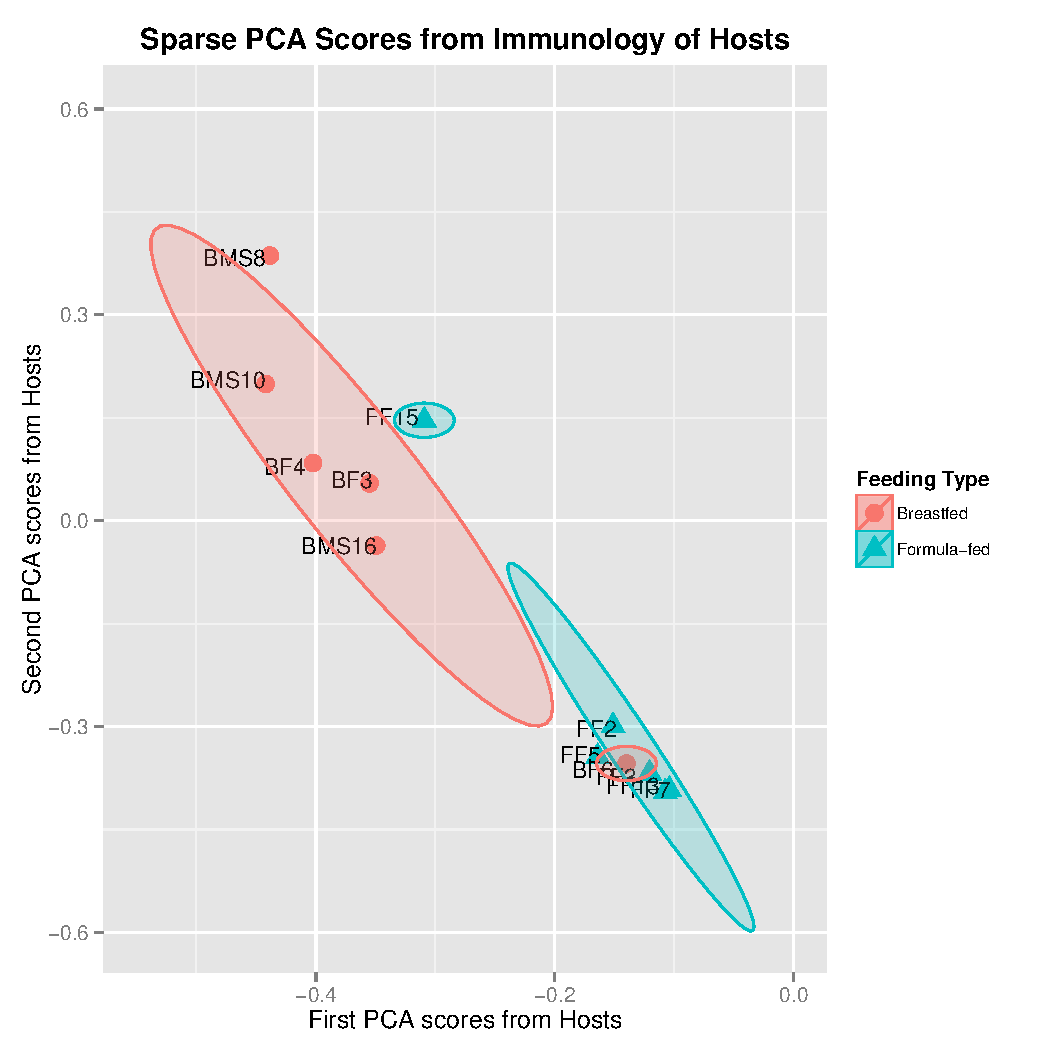
\includegraphics[width=\maxwidth]{figure/sparse_pca-1} 
\begin{kframe}\begin{alltt}
\hlcom{## sparse pca when microbial as base}
\hlstd{spca_seed_cv}\hlkwb{<-}\hlkwd{SPC.cv}\hlstd{(}\hlkwc{x}\hlstd{=cca_seed2,}\hlkwc{sumabsvs}\hlstd{=}\hlkwd{seq}\hlstd{(}\hlnum{1.2}\hlstd{,}\hlnum{12}\hlstd{,}\hlkwc{by}\hlstd{=}\hlnum{0.2}\hlstd{),}
                      \hlkwc{nfolds}\hlstd{=}\hlnum{10}\hlstd{,}\hlkwc{niter}\hlstd{=}\hlnum{10}\hlstd{)}
\end{alltt}
\begin{verbatim}
##  Fold  1  out of  10 
##  Fold  2  out of  10 
##  Fold  3  out of  10 
##  Fold  4  out of  10 
##  Fold  5  out of  10 
##  Fold  6  out of  10 
##  Fold  7  out of  10 
##  Fold  8  out of  10 
##  Fold  9  out of  10 
##  Fold  10  out of  10
\end{verbatim}
\begin{alltt}
\hlstd{spca_seed}\hlkwb{<-}\hlkwd{SPC}\hlstd{(}\hlkwc{x}\hlstd{=cca_seed2,}\hlkwc{sumabsv}\hlstd{=spca_seed_cv}\hlopt{$}\hlstd{bestsumabsv,}
                \hlkwc{K}\hlstd{=}\hlnum{2}\hlstd{)}
\end{alltt}
\begin{verbatim}
## 1234567
## 12345678910111213
\end{verbatim}
\begin{alltt}
\hlstd{spca_scores_seed}\hlkwb{<-}\hlstd{spca_seed}\hlopt{$}\hlstd{u}
\hlkwd{rownames}\hlstd{(spca_scores_seed)}\hlkwb{<-}\hlkwd{rownames}\hlstd{(cca_seed2)}
\hlstd{spca_scores_seed}\hlkwb{<-}\hlkwd{as.data.frame}\hlstd{(spca_scores_seed)}
\hlkwd{names}\hlstd{(spca_scores_seed)}\hlkwb{<-}\hlkwd{c}\hlstd{(}\hlstr{"microb1"}\hlstd{,}\hlstr{"microb2"}\hlstd{)}
\hlstd{spca_scores_seed}\hlopt{$}\hlstd{type}\hlkwb{<-}\hlkwd{c}\hlstd{(}\hlkwd{rep}\hlstd{(}\hlstr{"BF"}\hlstd{,}\hlnum{6}\hlstd{),}\hlkwd{rep}\hlstd{(}\hlstr{"FF"}\hlstd{,}\hlnum{6}\hlstd{))}

\hlcom{#ggplot of Sparse pca of microbial}
\hlstd{spca_plot2}\hlkwb{<-}\hlkwd{ggplot}\hlstd{(spca_scores_seed,}
                   \hlkwd{aes}\hlstd{(}\hlkwc{x}\hlstd{=microb1,}\hlkwc{y}\hlstd{=microb2,}\hlkwc{shape}\hlstd{=type,}\hlkwc{colour}\hlstd{=type))}
\hlstd{spca_plot2}\hlkwb{<-}\hlstd{spca_plot2}\hlopt{+}\hlkwd{geom_point}\hlstd{(}\hlkwc{size}\hlstd{=}\hlnum{4}\hlstd{)}
\hlstd{spca_plot2}\hlkwb{<-}\hlstd{spca_plot2}\hlopt{+}\hlkwd{scale_shape_discrete}\hlstd{(}\hlkwc{name}\hlstd{=}\hlstr{"Feeding Type"}\hlstd{,}
                                            \hlkwc{labels}\hlstd{=}\hlkwd{c}\hlstd{(}\hlstr{"Breastfed"}\hlstd{,}\hlstr{"Formula-fed"}\hlstd{))}
\hlstd{spca_plot2}\hlkwb{<-}\hlstd{spca_plot2}\hlopt{+}\hlkwd{scale_color_discrete}\hlstd{(}\hlkwc{name}\hlstd{=}\hlstr{"Feeding Type"}\hlstd{,}
                                            \hlkwc{labels}\hlstd{=}\hlkwd{c}\hlstd{(}\hlstr{"Breastfed"}\hlstd{,}\hlstr{"Formula-fed"}\hlstd{))}
\hlstd{spca_plot2}\hlkwb{<-}\hlstd{spca_plot2}\hlopt{+}\hlkwd{geom_text}\hlstd{(}\hlkwd{aes}\hlstd{(}\hlkwc{label}\hlstd{=}\hlkwd{rownames}\hlstd{(spca_scores_seed)),}
                                 \hlkwc{col}\hlstd{=}\hlstr{"black"}\hlstd{,}\hlkwc{hjust}\hlstd{=}\hlnum{1.1}\hlstd{,}\hlkwc{size}\hlstd{=}\hlnum{4}\hlstd{)}
\hlstd{spca_plot2}\hlkwb{<-}\hlstd{spca_plot2}\hlopt{+}\hlkwd{scale_x_continuous}\hlstd{(}\hlstr{"First PCA scores from Seedlevel2"}\hlstd{,}
                                          \hlkwc{limits}\hlstd{=}\hlkwd{c}\hlstd{(}\hlkwd{min}\hlstd{(spca_scores_seed[,}\hlnum{1}\hlstd{])}\hlopt{-}\hlnum{0.1}\hlstd{,}
                                                   \hlkwd{max}\hlstd{(spca_scores_seed[,}\hlnum{1}\hlstd{])}\hlopt{+}\hlnum{0.1}\hlstd{))}
\hlstd{spca_plot2}\hlkwb{<-}\hlstd{spca_plot2}\hlopt{+}\hlkwd{scale_y_continuous}\hlstd{(}\hlstr{"Second PCA scores from Seedlevel2"}\hlstd{,}
                                          \hlkwc{limits}\hlstd{=}\hlkwd{c}\hlstd{(}\hlkwd{min}\hlstd{(spca_scores_seed[,}\hlnum{2}\hlstd{])}\hlopt{-}\hlnum{0.1}\hlstd{,}
                                                   \hlkwd{max}\hlstd{(spca_scores_seed[,}\hlnum{2}\hlstd{])}\hlopt{+}\hlnum{0.1}\hlstd{))}
\hlstd{spca_plot2}\hlkwb{<-}\hlstd{spca_plot2}\hlopt{+}\hlkwd{labs}\hlstd{(}\hlkwc{title}\hlstd{=}\hlstr{"Sparse PCA Scores from Microbial Seedlevl2"}\hlstd{)}
\hlstd{spca_plot2}\hlkwb{<-}\hlstd{spca_plot2}\hlopt{+}\hlkwd{theme}\hlstd{(}\hlkwc{legend.title}\hlstd{=}\hlkwd{element_text}\hlstd{(}\hlkwc{size}\hlstd{=}\hlnum{10}\hlstd{),}
                             \hlkwc{legend.text}\hlstd{=}\hlkwd{element_text}\hlstd{(}\hlkwc{size}\hlstd{=}\hlnum{8}\hlstd{),}
                             \hlkwc{plot.title}\hlstd{=}\hlkwd{element_text}\hlstd{(}\hlkwc{size}\hlstd{=}\hlnum{14}\hlstd{,}\hlkwc{vjust}\hlstd{=}\hlnum{1.1}\hlstd{,}\hlkwc{face}\hlstd{=}\hlstr{"bold"}\hlstd{))}
\hlcom{## stat_ellipse has been sourced.}
\hlstd{spca_plot2}\hlkwb{<-}\hlstd{spca_plot2}\hlopt{+}\hlkwd{stat_ellipse}\hlstd{(}\hlkwd{aes}\hlstd{(}\hlkwc{x}\hlstd{=microb1,}\hlkwc{y}\hlstd{=microb2,}\hlkwc{fill}\hlstd{=type),}
                                    \hlkwc{level}\hlstd{=}\hlnum{0.6}\hlstd{,}\hlkwc{geom}\hlstd{=}\hlstr{"polygon"}\hlstd{,}\hlkwc{alpha}\hlstd{=}\hlnum{0.2}\hlstd{)}
\hlstd{spca_plot2}\hlkwb{<-}\hlstd{spca_plot2}\hlopt{+}\hlkwd{scale_fill_discrete}\hlstd{(}\hlkwc{name}\hlstd{=}\hlstr{"Feeding Type"}\hlstd{,}
                                            \hlkwc{labels}\hlstd{=}\hlkwd{c}\hlstd{(}\hlstr{"Breastfed"}\hlstd{,}\hlstr{"Formula-fed"}\hlstd{))}
\hlcom{#level for the scale of elli, alpha for the darkness of col,"polygon" for the cover of elli.}
\hlstd{spca_plot2}
\end{alltt}
\end{kframe}
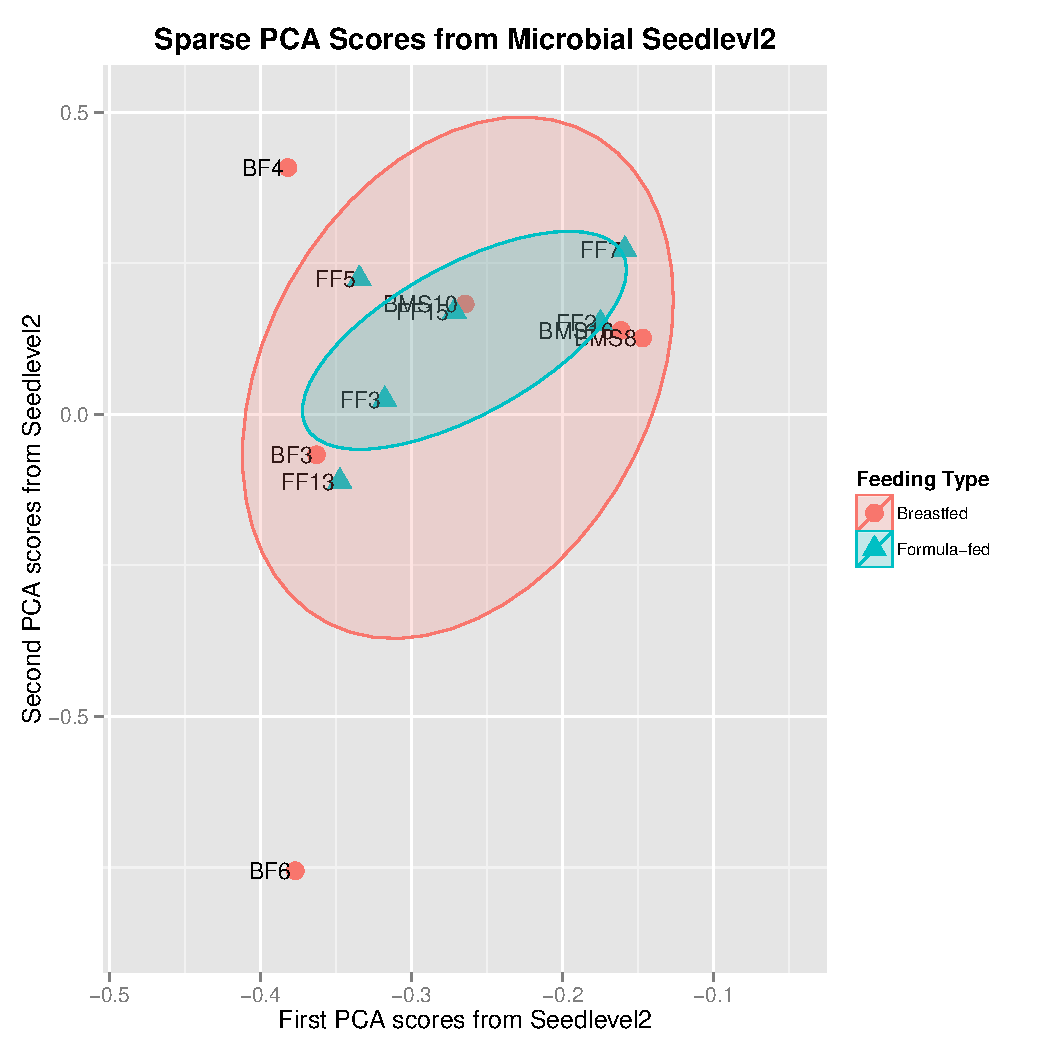
\includegraphics[width=\maxwidth]{figure/sparse_pca-2} 

\end{knitrout}
\end{document}
